%!TEX root = ../main.tex
I dette afsnit ses de forskellige Use cases. På figur~\ref{fig:fullydressedusecases} vises et Use Case diagram over de fully-dressed Use Cases, som viser de Use Cases, som er i fokus. 
\begin{figure}[H]
	\centering
	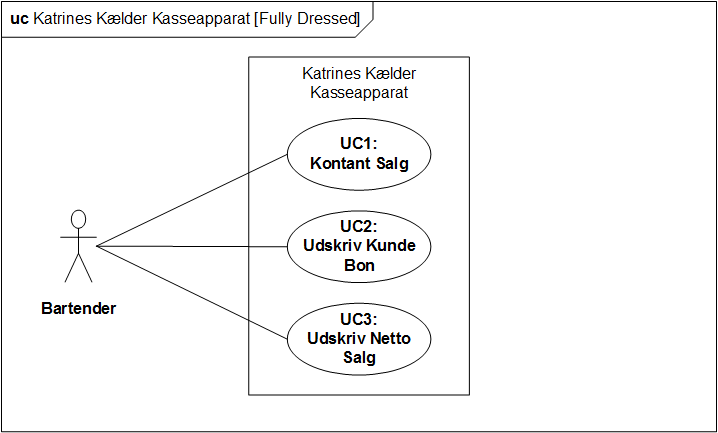
\includegraphics[width=0.6\textwidth]{Kravspecifikation/UseCases/UseCases_fully_dressed.png}
	\caption{Use-case diagram for de fully dressed use-cases.}
	\label{fig:fullydressedusecases}
\end{figure}

På figur~\ref{fig:ikkefullydressedusecases} vises et Use Case diagram over de ikke fully-dressed Use Cases, som ønskes implementeret på et senere tidspunkt. 

\begin{figure}[H]
	\centering
	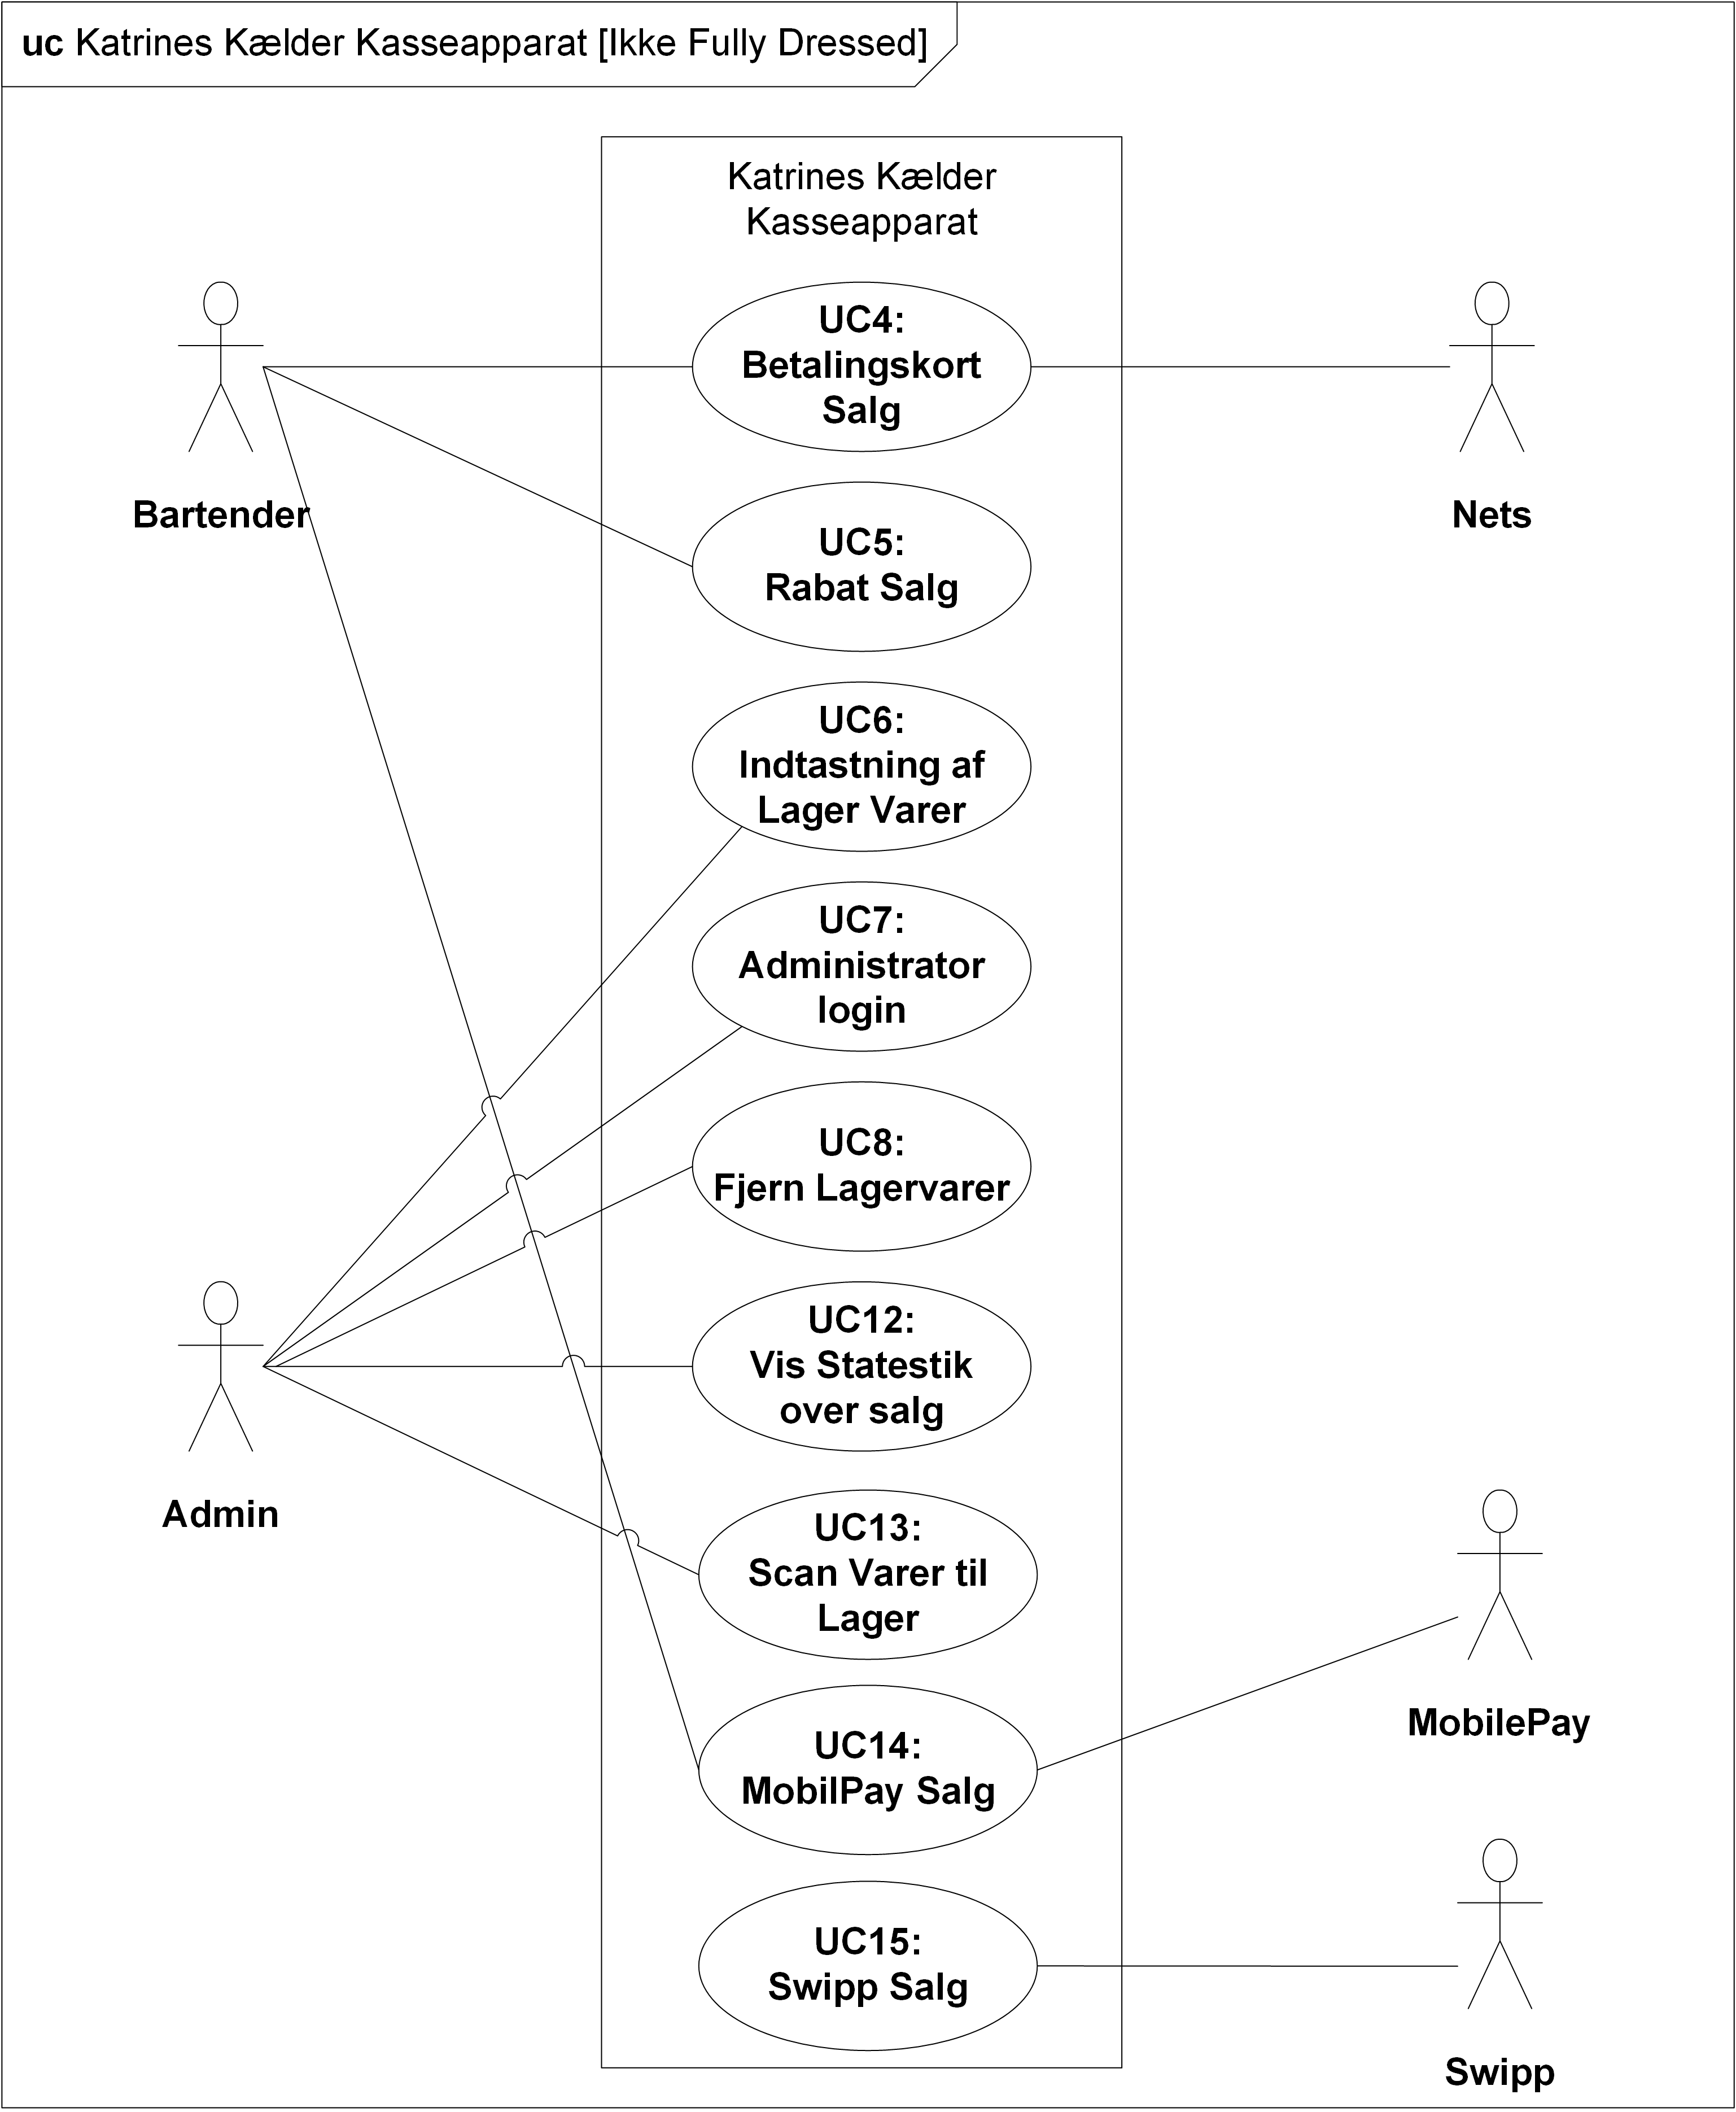
\includegraphics[width=0.6\textwidth]{Kravspecifikation/UseCases/UseCases_not_fully_dressed.png}
	\caption{Use Case diagram for de ikke fully dressed use-cases.}
	\label{fig:ikkefullydressedusecases}
\end{figure}

\newpage
%!TEX root = ../../main.tex

\subsection*{Use case 1}
I denne use case ser vi hvor et kontant salg bliver foretaget
\begin{usecase}{1}

\title{ Kontant Salg } 

\field{Mål:}{ At sælge drikkevarer mod kontant betaling }

\field{Initieret af:}{ Bartender }

\field{Aktører:}{ Bartender }

\field{Samtidige forekomster:}{1}

%Preconditions: What must be true on start and worth telling the reader?
\field{Prækondition:}{System skal være tændt og klar}

%Postconditions: What must be true on successful completion and worth telling the reader
\field{Postkondition:}{ Et kontant salg er foretaget }

%Main Success Scenario: A typical, unconditional happy path scenario of success.
\scenario{Hovedscenarie:}{
	\item Bartender vælger drink(s)/pris(er) på systemets touchskærm
	\item Bartender trykker "Total"	
	\item Den samlede pris udregnes
	\item Bartender trykker "Kontant" og skuffen åbnes
	\item Bartender modtager betaling fra kunden
	[Extension 1.1: Kontanter ikke modtaget]
	\item Købet er afsluttet
}


%Extensions: Alternate scenarios of success or failure.
\scenario{Extension 1.1: Kontanter ikke modtaget:}{
		\item Bartender trykker annuller køb
		\item Bartender lukker skuffen
		\item Systemet er klar til næste kunde
}


\end{usecase}


\newpage		
%!TEX root = ../../main.tex

\subsection*{Use case 1}
I denne use case -----
\begin{usecase}

\addtitle{Use Case 2}{ Udskriv Kundebon } 

\addfield{Mål:}{ Systemet får udskrevet en bon med kundens køb på }

\addfield{Initieret af:}{ Bartender }

\addfield{Aktører:}{ Bartender (Primær) }

\addfield{Samtidige forekomster:}{1}

%Preconditions: What must be true on start and worth telling the reader?
\addfield{Prækondition:}{Use Case 1 er gennemført}

%Postconditions: What must be true on successful completion and worth telling the reader
\addfield{Postkondition:}{Kunden (baretender?) modtager bon med køb på }

%Main Success Scenario: A typical, unconditional happy path scenario of success.
\addscenario{Hovedscenarie:}{
	\item Bartender har valgt at der skal udskrives bon (på GUI?)
	\item En dialogbox popper op og bartender bekræfter ønske af bon	
	\item printer udskriver bon  [Ext 1: Der er ikke mere papir]
	\item Bartender udleverer bon til kunde [Ext 2: Kunde er gået]	
}

%Extensions: Alternate scenarios of success or failure.
\addscenario{Udvidelser:}{
	\item[Ex.1] Der er ikke mere papir
		\begin{enumerate}
		\item[1.] Printer stopper. Dialogbox popper op med besked "Fyld papir på printer"
		\item[2.] Bartender fylder papir på printer.
		\item[3.] Der trykkes på 'OK' og fortsættes fra punkt 3
		\end{enumerate}
	\item[Ex.2] Kunde er gået
		\begin{enumerate}
			\item[1.] Bartender smider bon ud
		\end{enumerate}
}


\end{usecase}

\newpage
%!TEX root = ../../main.tex

\subsection*{Use case 3}
I denne use case, ses der hvordan der udskrives afstemning af kassen
\begin{usecase}{3}

\title{ Kasseafstemning } 

\field{Mål:}{ At Bartenderen har en bon med netto salg og dato udskrevet }

\field{Initieret af:}{ Bartender }

\field{Aktører:}{ Bartender }

\field{Samtidige forekomster:}{1}

%Preconditions: What must be true on start and worth telling the reader?
\field{Prækondition:}{System skal være tændt og klar}

%Postconditions: What must be true on successful completion and worth telling the reader
\field{Postkondition:}{ At netto salget på bonnen stemmer overens med salg indtastet }

%Main Success Scenario: A typical, unconditional happy path scenario of success.
\scenario{Hovedscenarie:}{
	\item Bartender vælger "Indstillinger"
	\item System viser "Indstillinger" menu
	\item Bartender trykker "Afstem"
	\item System viser "Afstem" popup
	[Extension 3.1: Bartender trykker "Annuller"]
	\item Bartender trykker "Godkend"
	\item Printeren printer bonnen
	\item System viser "Hovedmenu"
}


%Extensions: Alternate scenarios of success or failure.
\scenario{Extension 3.1: Bartender trykker Annuller:}{
		\item Systemet går tilbage til Indstillinger menu.
}


\end{usecase}
\newpage
\textbf{De moduler der realiserer Use Case 9: Tilføj varer til kasseapparat}

\begin{enumerate}
	\item Web API
	\item Database
	\item GUI
\end{enumerate}

Use Case 9 bliver realiseret primært gennem Web API'et som her bruger Database Controllere til at tilgå databasen. I Web API'et kan der indsættes nye produkter og det er samme database som den Business logikken henter i, hvortil der vises på GUI.

\newpage
\textbf{De Moduler der realiserer Use Case 10: Rediger varer i kasseapparat}

\begin{enumerate}
	\item Web API
	\item Database
	\item GUI
\end{enumerate}

Use Case 10 bliver realiseret primært gennem Wep API'et som her bruger Database Controllere til at tilgå databasen. I Wep API'et kan der redigeres i et allerede eksisterende produkt. Når et produkt er ændret som det ønskes, gemmes det i databasen, of da det er den samme database som business logikken henter fra, kan GUI'en vise det.
\newpage
\subsection*{Use Case 11}
I denne Use Case ser vi hvordan et produkt bliver fjernet fra databasen.
\begin{usecase}{11}

\title{ Fjern varer fra kasseapparat} 

\field{Mål:}{ At få slettet et produkt fra kasseapparatet }

\field{Initieret af:}{ Admin }

\field{Aktører:}{ Admin (Primær) }

\field{Samtidige forekomster:}{1}

%Preconditions: What must be true on start and worth telling the reader?
\field{Prækondition:}{Der skal være et produkt i databasen}

%Postconditions: What must be true on successful completion and worth telling the reader
\field{Postkondition:}{ Et produkt er slettet og vises ikke på GUI }

%Main Success Scenario: A typical, unconditional happy path scenario of success.
\scenario{Hovedscenarie:}{
	\item Admin vælger link til settings i Wep API
	\item Settings side vises og Admin vælger link til Products 
	\item Products side vises og Admin vælger produkt der skal slettes i produktlisten.
	\item Admin klikker på linket der fjerner produkter \newline
	[Extension 11.1: Admin klikker på andet end link til at fjerne produkt ]
	\item Produktet vises nu ikke i produktlisten
	\item Produktet vises ikke i GUI
}


%Extensions: Alternate scenarios of success or failure.
\scenario{Udvidelser:}{
	\item Extension 11.1: Admin klikker på andet end link til at fjerne produkt
		\begin{enumerate}
		\item[1.] Systemet går ud af produkt side og en anden side vises
		\end{enumerate}		
}


\end{usecase}
\newpage
\subsection*{Use Case 12}
I denne Use Case ser vi hvordan der vises statistik over solgte produkter i systemet.
\begin{usecase}{12}

\title{ Vis statistik over salg} 

\field{Mål:}{ At få vist statistik over solgte produkter }

\field{Initieret af:}{ Admin }

\field{Aktører:}{ Admin (Primær) }

\field{Samtidige forekomster:}{1}

%Preconditions: What must be true on start and worth telling the reader?
\field{Prækondition:}{Der skal mindt være en igangværende ordre}

%Postconditions: What must be true on successful completion and worth telling the reader
\field{Postkondition:}{ Der vises statistik af solgte produkter og ordrer }

%Main Success Scenario: A typical, unconditional happy path scenario of success.
\scenario{Hovedscenarie:}{
	\item Admin vælger link til Statistik i Wep API
	\item Statistik side vises og Admin vælger ordrer i ordrerlisten
	\item Admin klikker på linket til detaljer om en ordre og detaljer om ordre vises.
	\newline
	[Extension 1.1: Admin klikker på andet end link til at tilføje produkt ]	
}


%Extensions: Alternate scenarios of success or failure.
\scenario{Udvidelser:}{
	\item Extension 1.1: Admin klikker på andet link end link til detaljer
		\begin{enumerate}
		\item[1.] Systemet går ud af produkt side og en anden side vises
		\end{enumerate}		
}


\end{usecase}
\newpage
\section{Ikke fully dressed use cases}

\subsubsection*{Use Case 4 - Dankort Salg}
skal beskrive forløbet for et salg når kasseapparatet interagerer med dankort automaten.

\subsubsection*{Use Case 5 - Medarbejder Salg}
Heri beskrives forløbet for salg til en medarbejder der opnår rabat.

\subsubsection*{Use Case 6 - Indtastning af lager varer}
Til lagerstyrings delen af produktet skal der være mulighed for at indtaste vare i systemet når de ankommer/bestilles.

\subsubsection*{Use Case 7 - Admin login}
For at kunne ændre priser, indsætte nye varer osv. skal der kunne logges ind på en administrationsdel af systemet således at ikke alle og enhver kan gøre dette.

\subsubsection*{Use Case 8 - Fjern lagervarer}
Når der hentes varer på lageret skal disse kunne tjekkes ud af systemet.

\subsubsection*{Use Case 9 - Tilføj varer til kasseapparat}
Det skal være muligt at tilføje en varer til kasseapparatet denne use case kræver at admin login use casen er udført.

\subsubsection*{Use Case 10 - Rediger varer i kasseapparat}
Det skal være muligt at ændre en varers pris og navn osv. denne use case kræver admin login use casen er udført.

\subsubsection*{Use Case 11 - Fjern varer fra kasseapparat}
Det skal være muligt at fjerne drinks fra systemet hvis de f.eks. ikke længere bliver serveret. denne use case kræver admin login use casen er udført.

\subsubsection*{Use Case 12 - Vis Statistik over salg}
Der skal kunne generes en statistik over de varer der er blevet solgt gerne i detaljer der specifikt beskriver hvilke drinks der er solgt.

\subsubsection*{Use Case 13 - Scan varer til lager}
Der skal kunne bruges et apparat der kan scanne varer ind i lager systemet. 
